\documentclass[svgnames,11pt]{beamer}
\input{/home/tof/Documents/Cozy/latex-include/preambule_commun.tex}
\input{/home/tof/Documents/Cozy/latex-include/preambule_beamer.tex}
%\usepackage{pgfpages} \setbeameroption{show notes on second screen=left}
\author[]{Christophe Viroulaud}
\title{Dessiner avec turtle}
\date{\framebox{\textbf{Lang 04}}}
%\logo{}
\institute{Première - NSI}

\begin{document}
\begin{frame}
\titlepage
\end{frame}
\begin{frame}
    \frametitle{}

    Pour faciliter le travail des développeurs Python, il existe des outils spécialisés dans diverses tâches. On les appelle \emph{bibliothèques}, \emph{modules} ou encore \emph{librairies}. Comme son nom l'indique la bibliothèque \textbf{\texttt{math}} offre des fonctionnalités permettant d'effectuer des calculs mathématiques.
\begin{center}
    \framebox{Comment utiliser une bibliothèque?}
\end{center}
\end{frame}
\section{La documentation}
\begin{frame}
    \frametitle{La documentation}

    Il n'est pas nécessaire de connaître par cœur toutes les possibilités de chaque librairie. Il est par contre indispensable de savoir utiliser la documentation en ligne de Python.

\end{frame}
\begin{frame}
    \frametitle{}

    \begin{activite}
        \begin{enumerate}
            \item Se rendre sur la page \url{https://docs.python.org/3/}
            \item Sélectionner la langue et la version de Python correspondante à l'EDI utilisé.
            \item Dans la barre de recherche, taper \textbf{\texttt{math}} et ouvrir le premier lien.
            \item Chercher la fonction permettant de calculer la racine carrée d'un nombre.
            \end{enumerate}
    \end{activite}

\end{frame}
\begin{frame}
    \frametitle{Avant de regarder la correction}
\begin{center}
    \centering
    \includegraphics[width=3cm]{/home/tof/Documents/Cozy/latex-include/stop.png}
    \end{center}
{\Large
    \begin{itemize}
        \item Prendre le temps de réfléchir,
        \item Analyser les messages d'erreur,
        \item Demander au professeur.
    \end{itemize}
}
\end{frame}
\begin{frame}[fragile]
    \frametitle{Correction}

\begin{center}
\begin{lstlisting}[language=Python , basicstyle=\ttfamily\small, xleftmargin=2em, xrightmargin=2em]
from math import sqrt
print(sqrt(25))
\end{lstlisting}
\captionof{code}{Racine carré}
\label{CODE}
\end{center}

\end{frame}
\section{Importation}
\begin{frame}
    \frametitle{Importation}

    Pour utiliser les fonctionnalités proposées par une bibliothèque, il faut d'abord l'importer dans le programme. Plusieurs possibilités d'import existent.

\end{frame}
\begin{frame}[fragile]
    \frametitle{}
\begin{lstlisting}[language=Python , basicstyle=\ttfamily\small, xleftmargin=1em, xrightmargin=1em]
# importe toute la bibliothèque
import math
# calcule le cosinus de l'angle (en radians)
c = math.cos(0.5)
\end{lstlisting}
\begin{lstlisting}[language=Python , basicstyle=\ttfamily\small, xleftmargin=1em, xrightmargin=1em]
# importe toute la bibliothèque et lui donne un alias
import math as m
c = m.cos(0.5)
\end{lstlisting}
\end{frame}
\begin{frame}[fragile]
    \frametitle{}

    \begin{lstlisting}[language=Python , basicstyle=\ttfamily\small, xleftmargin=1em, xrightmargin=1em]
# importe toutes les fonctions de la bibliothèque
from math import *
# Il ne faut plus faire référence au nom de la bibliothèque
c = cos(0.5)
\end{lstlisting}
\begin{lstlisting}[language=Python , basicstyle=\ttfamily\small, xleftmargin=1em, xrightmargin=1em]
# n'importe que les fonctions nécessaires dans le programme
from math import cos
# Il ne faut plus faire référence au nom de la bibliothèque
c = cos(0.5)
\end{lstlisting}
\end{frame}
\begin{frame}
    \frametitle{}

    \begin{activite}
    \begin{enumerate}
        \item Écrire un programme qui renvoie le cosinus, le sinus et la valeur en degrés d'un angle $\frac{\pi}{2}$.
        \item Comment expliquer la valeur du cosinus?
    \end{enumerate}
    \end{activite}

\end{frame}
\begin{frame}
    \frametitle{Avant de regarder la correction}
\begin{center}
    \centering
    \includegraphics[width=3cm]{/home/tof/Documents/Cozy/latex-include/stop.png}
    \end{center}
{\Large
    \begin{itemize}
        \item Prendre le temps de réfléchir,
        \item Analyser les messages d'erreur,
        \item Demander au professeur.
    \end{itemize}
}
\end{frame}
\begin{frame}[fragile]
    \frametitle{Correction}

\begin{center}
\begin{lstlisting}[language=Python , basicstyle=\ttfamily\small, xleftmargin=2em, xrightmargin=2em]
from math import cos, sin, degrees, pi

angle = pi/2
print("en degré:", degrees(angle))
print("cos: ", cos(angle))
print("sin: ", sin(angle))    
\end{lstlisting}
\captionof{code}{Trigonométrie}
\label{CODE}
\end{center}
Mathématiquement $\cos\frac{\pi}{2}=0$. La représentation des nombres réels en mémoire peut poser problème.
\end{frame}
\section{Une bibliothèque graphique}
\subsection{Découverte}
\begin{frame}
    \frametitle{Découverte}

    La bibliothèque \textbf{\texttt{turtle}} est un module simple pour réaliser des figures géométriques. La \emph{tortue} avance, tourne sur l'écran et trace les traits demandés par l'utilisateur.

\end{frame}
\subsection{Premiers déplacements}
\begin{frame}
    \frametitle{Premiers déplacements}

    Les possibilités sont nombreuses. Il faut d'abord découvrir quelques déplacements.
    \begin{activite}
        \begin{enumerate}
        \item Dans la documentation, chercher le rôle des fonctions:
        \begin{itemize}
        \item \texttt{\textbf{forward, backward}}
        \item \texttt{\textbf{left, right}}
        \item \texttt{\textbf{up, down}}
        \end{itemize}
        \item Tracer un carré de 100 de côté.
        \end{enumerate}
        \end{activite}
\end{frame}
\begin{frame}
    \frametitle{Avant de regarder la correction}
\begin{center}
    \centering
    \includegraphics[width=3cm]{/home/tof/Documents/Cozy/latex-include/stop.png}
    \end{center}
{\Large
    \begin{itemize}
        \item Prendre le temps de réfléchir,
        \item Analyser les messages d'erreur,
        \item Demander au professeur.
    \end{itemize}
}
\end{frame}
\begin{frame}[fragile]
    \frametitle{Correction}

\begin{center}
\begin{lstlisting}[language=Python , basicstyle=\ttfamily\small, xleftmargin=2em, xrightmargin=2em]
import turtle as t

for _ in range(4):
    t.forward(100)
    t.left(90)
t.done()
\end{lstlisting}
\captionof{code}{Carré}
\label{CODE}
\end{center}

\end{frame}
\subsection{Des figures plus complexes}
\begin{frame}
    \frametitle{Des figures plus complexes}

    \begin{activite}
        \begin{enumerate}
        \item Réaliser la figure \ref{carres}.
        \item Remplir chaque carré avec une couleur, de la manière suivante:
        \begin{itemize}
        \item rouge si le numéro du carré tracé est impair,
        \item vert s'il est pair.
        \end{itemize}
        \end{enumerate}
        \end{activite}
        \begin{figure}[!h]
        \centering
        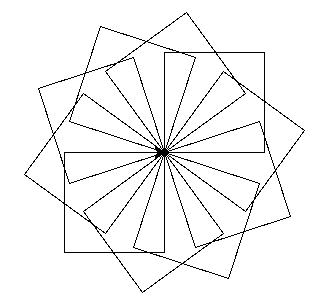
\includegraphics[width=4cm]{ressources/carres.png}
        \captionof{figure}{Des carrés et des rotations}
        \label{carres}
        \end{figure}

\end{frame}
\begin{frame}
    \frametitle{Avant de regarder la correction}
\begin{center}
    \centering
    \includegraphics[width=3cm]{/home/tof/Documents/Cozy/latex-include/stop.png}
    \end{center}
{\Large
    \begin{itemize}
        \item Prendre le temps de réfléchir,
        \item Analyser les messages d'erreur,
        \item Demander au professeur.
    \end{itemize}
}
\end{frame}
\begin{frame}[fragile]
    \frametitle{Correction}

\begin{center}
\begin{lstlisting}[language=Python , basicstyle=\ttfamily\small, xleftmargin=1em, xrightmargin=1em]
import turtle as t

for i in range(10):
    # on trace le carré
    for j in range(4):
        t.forward(100)
        t.left(90)

    # on tourne de 36° pour faire le tour complet
    t.left(36)

t.done()
\end{lstlisting}
\captionof{code}{Rosaces}
\label{CODE}
\end{center}   

\end{frame}
\begin{frame}[fragile]
    \frametitle{Correction}

\begin{center}
\begin{lstlisting}[language=Python , basicstyle=\ttfamily\small, xleftmargin=1em, xrightmargin=1em]
for i in range(10):
    # i est pair (le reste de la division par 2 est nul)
    if i%2 == 0:
        t.color("green", "green")
    else:
        t.color("red", "red")

    t.begin_fill()
    for j in range(4):    # on trace le carré
        t.forward(100)
        t.left(90)

    t.end_fill()
    t.left(36)
t.done()
\end{lstlisting}
\captionof{code}{Rosaces colorées}
\label{CODE}
\end{center}

\end{frame}
\begin{frame}
    \frametitle{Code complet}

    Le code complet est accessible \href{https://cviroulaud.github.io/premiere/langages/dessiner-avec-turtle/scripts/turtle.zip}{ici}.

\end{frame}
\end{document}